\chapter{Revisão Bibliográfica}

Nesse capítulo será apresentada uma revisão bibliográfica dos tópicos concernentes a acústica interna de dutos circulares. Os tópicos estão separados em modelos analíticos exatos, modelos analíticos aproximados, trabalhos experimentais, modelos numéricos e trabalhos relacionados ao desenvolvimento e aplicação do método de \textit{lattice} Boltzmann para problemas de acústica.

\section{Modelos Analíticos Exatos} 

A propagação de modos normais (ondas planas) é um problema clássico em acústica e continua tendo importância significativa mediante ao advento de novas tecnologias relacionadas a sistemas de exaustão e sucção. Em geral, pode-se utilizar dois parâmetros para caracterizar o fenômeno da acústica interna de dutos:

\begin{itemize}
    \item a magnitude do coeficiente de reflexão $R_{r}$, razão entre as componentes refletida e incidente da onda no duto, a qual é dada por
    \begin{equation}
        R_{r}\simbolo{$R_{r}$}{Coeficiente de reflexão na terminação do duto} =\frac{Z_{r} - Z_{0}}{Z_{r} + Z_{0}},
        \label{eq:R}
    \end{equation}
    sendo $Z_{r}$\simbolo{$Z_{r}$}{Impedância de radiação} a impedância de radiação e $Z_{0}$\simbolo{$Z_{0}$}{Impedância característica do meio} a impedância característica do meio, definida por $Z_{0} = \rho_{0}c_{0}$, tal que $\rho_{0}$ e $c_{0}$ são, respectivamente, as constantes de densidade média do meio\simbolo{$\rho_{0}$}{Densidade média do meio} e velocidade do som\simbolo{$c_{0}$}{Velocidade do som};
    
    \item coeficiente de correção da terminação normalizado pelo raio do duto $l/a$ em que $a$ é o raio do duto. Tal parâmetro representa o comprimento acústico efetivo do duto. Em outras palavras, o fator $l$ é a quantidade adicional medida a partir da abertura do duto a qual deve propagar a onda incidente antes de ser refletida para o interior do duto com fase invertida. Tal coeficiente de correção da terminação $l$ é dado por
    \begin{equation}
        l = \frac{1}{k} \arctan\!\left(\frac{Z_{r}}{Z_{0} \, \mathrm{j}\simbolo{$j$}{Unidade imaginária}}\right)
        \label{eq:l}
    \end{equation}
    sendo $k$\simbolo{$k$}{Número de onda} o número de onda.
\end{itemize}

Em relação aos parâmetros discutidos acima, a solução exata para o problema de um duto não flangeado na ausência de escoamento foi proposta por \citeonline{levine1948radiation}, porém em boa parte das aplicações práticas dutos transportam escoamentos médios. Para tais circunstâncias, \citeonline{munt1990acoustic} propôs um modelo analítico exato, também baseado na técnica de Wiener-Hopf, em que se considera a presença de um escoamento subsônico no interior do duto. Considera-se nesse modelo as premissas de que o escoamento é uniforme, invíscido e que a camada cisalhante do jato é infinitamente fina. Além disso, o modelo considera a condição de Kutta na borda do duto para lidar com a singularidade da velocidade de partícula nesta região. As Figuras \ref{fig:comp1} e \ref{fig:comp2} apresentam as comparações entre casos com e sem escoamento para um duto não flangeado em termos de $R_{r}$ e $l/a$.

\begin{figure}[ht!]
\centering
  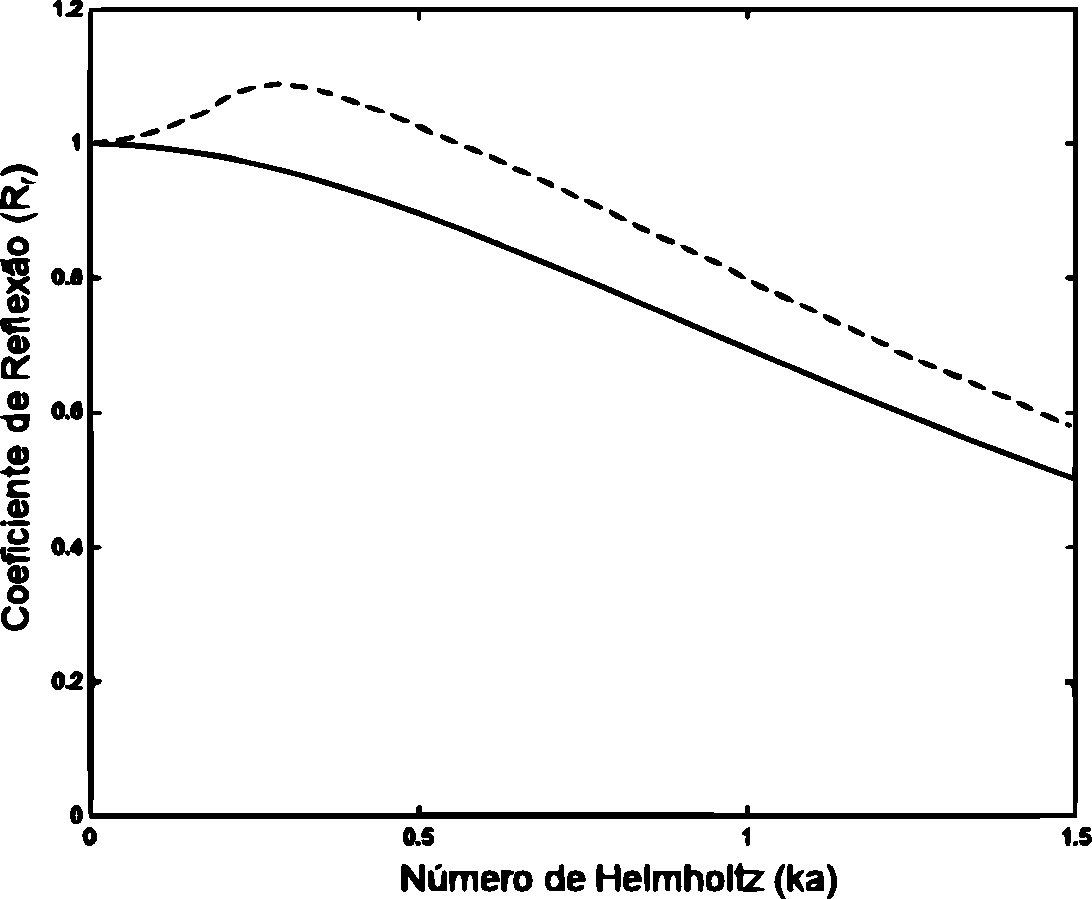
\includegraphics[width=.9\linewidth]{figuras/abs_r_comparacao.pdf}
  \caption[Magnitudes do coeficiente de reflexão $R_{r}$]{Resultados analíticos exatos para magnitude do coeficiente de reflexão $R_{r}$ ao final de um duto não flangeado. A linha contínua apresenta o resultado sem escoamento de \citeonline{levine1948radiation} e a linha tracejada apresenta o resultado com escoamento de Mach = 0,15 de \citeonline{munt1990acoustic}.}
  \label{fig:comp1}
\end{figure}

\newpage
Como é mostrado na Figura \ref{fig:comp1}, a magnitude do coeficiente de reflexão $R_{r}$ aumenta consideravelmente na presença de um escoamento subsônico. Além disso, pode-se perceber que, em algumas frequências, $R_{r}$ torna-se maior do que a unidade, implicando que a amplitude da onda refletida torna-se maior do que a da onda incidente. Este fenômeno ocorre, sobretudo, pela interação do escoamento com a borda do duto, a qual transforma energia cinética rotacional em energia acústica, como discutido por \citeonline{peters1993}. Além disso vale ressaltar que o maior valor de $R_{r}$ está associado com a frequência de desprendimento de vórtices na saída do duto, ou seja, a um número de Strouhal ($St$) relativo a maximização do desprendimento de vórtices na terminação do duto.  

\begin{figure}[ht!]
\centering
  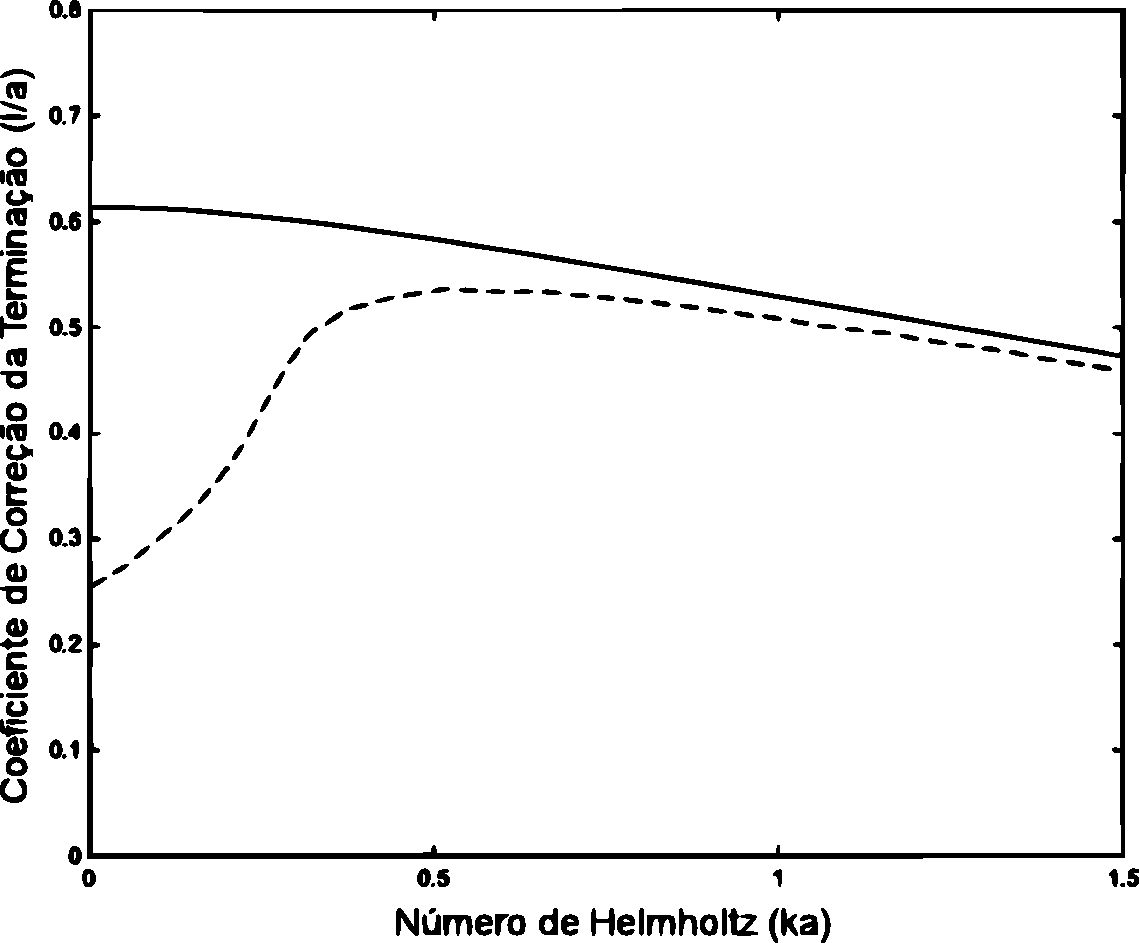
\includegraphics[width=.9\linewidth]{figuras/loa_comparacao.pdf}
  \caption[Coeficientes de correção de terminação $l/a$]{Resultados analíticos exatos para o coeficiente de correção da terminação normalizado pelo raio $l/a$ de um duto não flangeado. A linha contínua apresenta o resultado sem escoamento de \citeonline{levine1948radiation} e a linha tracejada apresenta o resultado com escoamento de Mach = 0,15 de \citeonline{munt1990acoustic}.}
  \label{fig:comp2}
\end{figure}

\newpage
De acordo com a Figura \ref{fig:comp2}, a correção normalizada da terminação $l/a$ torna-se consideravelmente menor do que aquela obtida na ausência de escoamento, sobretudo para baixos números de Helmholtz ($ka$)\simbolo{$ka$}{Número de Helmholtz}. Em outras palavras, para baixas frequências e na presença de um escoamento a onda acústica é refletida em uma região mais próxima da abertura, em comparação à situação sem escoamento.

\section{Modelos Analíticos Aproximados}

No que diz respeito a modelos analíticos aproximados, o trabalho de \citeonline{carrier1955sound} foi um dos primeiros a abordar o cálculo do coeficiente de reflexão e correção da terminação com escoamento de exaustão num duto não flangeado. Para tal foi considerado um gás perfeito invíscido com o tipo de escoamento uniforme (\textit{plug}). Nessa abordagem usou-se a mesma metodologia que \citeonline{levine1948radiation} porém acoplando à formulação matemática o método de Prandtl-Glauert. Esse modelo é limitado a Machs subsônicos ($M$ $<$ $0,4$)\simbolo{$M$}{Número de Mach} e ondas planas, ou seja, valores de $ka$ $<$ $1,8$.

\citeonline{mani1973refraction} deu continuidade a mesma abordagem de \citeonline{carrier1955sound} com escoamento de exaustão para Machs subsônicos ($M$ $<$ $0,3$) e ondas planas, porém considerando deslocamento transversais de partículas na interface entre o ar em repouso externo e o jato de saída do duto como condição de cortorno do problema. Esse tipo de solução mostra diversos fenômenos antes não previstos com os outros modelos citados como efeitos de convecção, zonas de silêncio relativo e refrações.

Também na mesma linha de desenvolvimento de \citeonline{carrier1955sound}, \citeonline{savkar1975radiation} desenvolveu um modelo de modos de alta ordem ($ka$ $<$ $4,59$) com escoamento de exaustão e sucção do tipo \textit{plug} ($M$ $<$ $0,4$) com variação de temperatura. A continuidade do deslocamento das partículas acústicas transversais também foi considerada na interface entre o ar em repouso externo e o jato de saída do duto, possibilitando assim análises de fenômenos de convectivos. Como metodologia para construção desse modelo foram aplicadas as técnicas de Wiener-Hopf e a aproximação matemática do trabalho de \citeonline{carrier1955sound}.

Já o trabalho de \citeonline{hirschberg2014} propõe uma expressão analítica aproximada do coeficiente de reflexão para baixas frequências ($ka$ $<$ $1$) e para baixos números de Mach ($M$ $<$ $0,2$). Esse modelo considera os efeitos de convecção e temperatura e foi consolidado a partir da aproximação proposta pelo trabalho de \citeonline{howe1979}.   

\section{Trabalhos Experimentais}

\subsection{Escoamento Sugado}

Em relação a trabalhos experimentais, \citeonline{ingard1975} investigaram o coeficiente de reflexão em dutos quadrados em regime de escoamento succionado de Mach 0,4. O método de medição se baseou na técnica de dois microfones e os mesmos foram ajustados para números de Helmholtz ($ka$) menores que 0,5. Em vista desse contexto experimental, o autor desenvolveu uma fórmula analítica para o cálculo do coeficiente de reflexão para baixas frequências.

Na mesma linha de investigação, \citeonline{davies1987} investigou o coeficiente de reflexão para baixas frequências ($0,01$ $<$ $ka$ $<$ $0,25$) e Machs subsônicos ($M$ $<$ $0,3$), porém com dutos circulares não flangeados e flangeados. O autor destaca que a disposição geométrica da terminação do duto, quando submetida a fenômenos de escoamentos succionados, desenvolve a chamada \textit{vena} contracta, que pode ser estimada e associada com o fator de perda $Kp$\simbolo{$Kp$}{Fator de perda}. Em vista dos procedimentos desse trabalho, o autor compara os resultados com o estudo de \citeonline{ingard1975} e sugere um aperfeiçoamento na equação analítica do cálculo do coeficiente de reflexão.

Dos trabalhos citados com escoamento sugado nota-se a consolidação do comportamento do coeficiente de reflexão para baixas frequências. Esse comportamento ocorre pelo surgimento de uma \textit{vena} contracta, descolamento de fluido da parede do duto que, dependendo do número de Mach, se estende mais ou menos para dentro do duto. De acordo com o trablaho de \citeonline{davies1987}, para baixas frequências ($ka$ $<$ $0,25$) o coeficiente de reflexão muda com relação ao Mach e é modelado de acordo com a equação
    \begin{equation}
        R_{M}\simbolo{$R_{M}$}{Coeficiente de reflexão em relação ao Mach} = R_{0}\bigg[\frac{(1 - M)}{(1 + M)}\bigg]^{0,9},
        \label{eq:R_M}
    \end{equation}
    sendo $R_{0}$ módulo do coeficiente de reflexão sem escoamento obtido a partir do trabalho de \citeonline{levine1948radiation}. 



    De forma análoga o trabalho de \citeonline{davies1987} também sugere uma equação para o coeficiente de correção da terminação e a mesma é definida por
    \begin{equation}
        l_{M}\simbolo{$l_{M}$}{Coeficiente de correção da terminação em relação ao Mach} = l_{0}(1 - M^{2}),
        \label{eq:l_M}
    \end{equation} 
    sendo $l_{0}$ módulo do coeficiente de correção da terminação sem escoamento obtido a partir do trabalho de \citeonline{levine1948radiation}.


\begin{figure}[h!]
\centering
  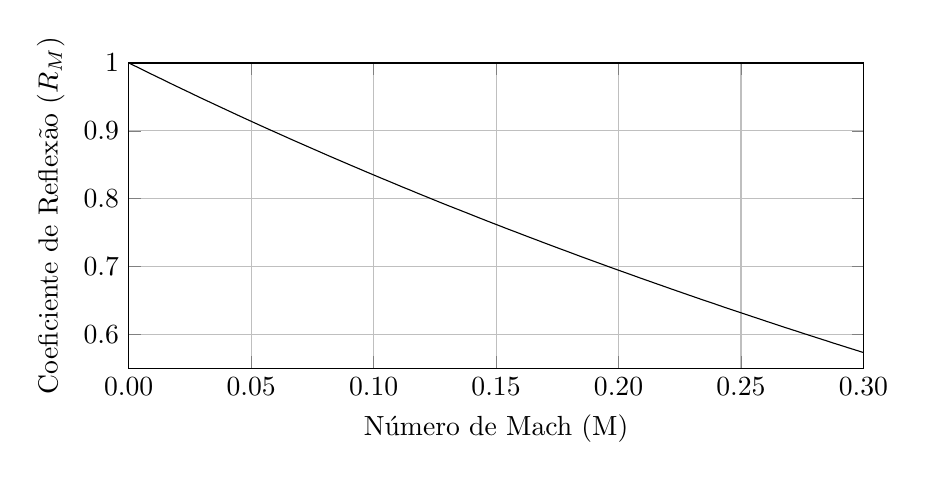
\begin{tikzpicture}
  \begin{axis}[
      %axis lines = left,
      xlabel = Número de Mach (M),
      ylabel = Coeficiente de Reflexão ($R_{M}$),
      width=0.9\textwidth,
      height=0.45\textwidth,
      ytick distance=0.1,
      x tick label style={
        /pgf/number format/.cd,
            fixed,
            fixed zerofill,
            precision=2,
        /tikz/.cd
    },
    xmin=0,
    xmax=0.3,
    ymin=0.55,
    ymax=1,
    grid=major
  ]
  %Below the red parabola is defined
  \addplot [
      domain=0:0.3, 
      samples=100, 
      color=black
  ]
  {((1 - x)/(1 + x))^0.9};
   
  \end{axis}
  \end{tikzpicture}
  \caption[Coeficiente de reflexão $R_{M}$]{Resultado do coeficiente de reflexão $R_{M}$ em relação ao Mach para baixas frequências ($ka$ $<$ $0,25$). A linha tracejada apresenta o cálculo obtido com a equação \ref{eq:R_M} do trabalho de \citeonline{davies1987}.}
  \label{fig:comp3}
\end{figure}

A Figura \ref{fig:comp3} mostra o gráfico resultante da equação \ref{eq:R_M} e pode-se perceber que $R_{M}$ decai de acordo com o aumento do Mach, em outras palavras, para baixas frequências, a onda plana possui maior facilidade de se radiar para o meio externo a medida que o Mach é aumentado. 


\begin{figure}[h!]
\centering
  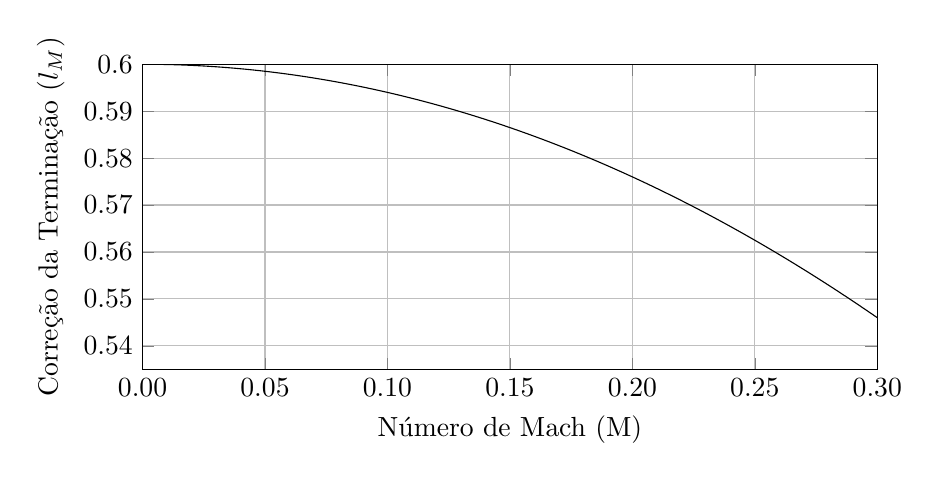
\begin{tikzpicture}
  \begin{axis}[
      %%axis lines = left,
      xlabel = Número de Mach (M),
      ylabel = Correção da Terminação ($l_{M}$),
      width=0.9\textwidth,
     height=0.45\textwidth,
      ytick distance=0.01,
       x tick label style={
        /pgf/number format/.cd,
            fixed,
            fixed zerofill,
            precision=2,
        /tikz/.cd,
    },
    xmin=0,
    xmax=0.3,
    ymin=0.535,
    ymax=0.6,
    grid=major
  ]
  %Below the red parabola is defined
  \addplot [
      domain=0:0.3, 
      samples=100, 
      color=black
  ]
  {0.6*(1 - x^2)};
   
  \end{axis}
  \end{tikzpicture}
  \caption[Coeficiente de correção da terminação $l_{M}$]{Resultado do coeficiente de correção da terminação $l_{M}$ em relação ao Mach para baixas frequências ($ka$ $<$ $0,25$). A linha tracejada apresenta o cálculo obtido com a equação \ref{eq:l_M} do trabalho de \citeonline{davies1987}.}
  \label{fig:comp4}
\end{figure}

 A Figura \ref{fig:comp4} mostra o gráfico resultante da equação \ref{eq:l_M} e pode-se perceber que $l_{M}$ decai de acordo com o aumento do Mach, ou seja, para baixas frequências, o comprimento efetivo acustico do duto diminui a medida que o Mach é aumentado. Mesmo com esses coeficientes modelados com apoio de dados experimentais a literatura carece de informações sobre esses parâmetros para frequências mais altas ($ka$ $>$ $0,25$).


\subsection{Escoamento de Exaustão}

No que diz respeito a escoamentos de exaustão o trabalho de \citeonline{peters1993} investigou os coeficientes de reflexão e de dissipação de ondas acústicas devido aos efeitos térmicos e de viscosidade. Uma técnica multi-microfones, baseada na técnica de dois microfones, foi utilizada para extração dos dados num regime de baixas frequências ($ka$ $<$ $1,5$) e Machs subsônicos ($M$ $<$ $0,2$). Por fim o autor argumenta que o fenômeno do coeficiente de reflexão ser maior que o valor unitário ocorre devido a interação do escoamento com a borda do duto, a qual transforma energia cinética rotacional em energia acústica. 

O trabalho de \citeonline{allam2006investigation} utilizou um sistema superdeterminado de medição para investigação da acústica interna de um duto não flangeado. Para contornar a dificuldade de medição do coeficiente de correção da terminação do duto, surgiu-se como motivação o desenvolvimento de um sistema em que há mais microfones do que incógnitas a serem calculadas, em outras palavras, extendeu-se a metodologia de medição de 2 microfones para mais que 4 microfones. Há de se considerar também que a parte imaginária do número de onda, parte associada com a dissipação de energia por viscosidade, não pode ser obtida quando há escoamento e por isso foi incluída como incógnita. Em linhas gerais esse trabalho permitiu a validação experimental do trabalho de \citeonline{munt1990acoustic} e a consolidação de um sistema confiável de medição para esse tipo de problema.

\citeonline{english2010} investigou também de forma experimental os coeficientes de reflexão e de terminação de dutos circulares com diferentes espessuras, através da técnica de extração de autoespectro e espectro cruzado em pares de microfones calibrados para o intervalo $0$ $<$ $ka$ $<$ $0,7$. Focando para números de Mach entre 0 e 0,3, seus resultados mostram que os coeficientes de reflexão estão com valores acima dos que são encontrados no trabalho de \citeonline{munt1990acoustic} e \citeonline{allam2006investigation}. O autor explica esse fato relatando que a condição de Kutta subestima o surgimento de vórtices na saída do duto bem como a influência da espessura da parede do duto diferente do experimento de \citeonline{allam2006investigation}.

Já o trabalho de \citeonline{tiikoja2014} focou na validação do modelo de \citeonline{munt1990acoustic} e a investigação da influência de jatos quentes (temperatura de até $200^{o}$ $C$) nos coeficientes de reflexão e de terminação de dutos circulares. Para tal fim utilizaram a técnica de 2 microfones num sistema superdeterminado com 3 microfones, ajustados num contexto de ondas planas ($ka$ $<$ $1,8$) e Machs de até 0,3 e 0,12 para jatos frios e quentes respectivamente. Tendo como referências as curvas validadas de jatos frios de \citeonline {munt1990acoustic}, foi observado como resultado do estudo que para jatos quentes as curvas dos coeficientes de reflexão e de terminação sofrem um aumento de amplitude e um deslocamento em direção para baixas frequências.


\section{Modelos Numéricos}

Já em relação a trabalhos envolvendo métodos numéricos, \citeonline{selamet2001wave} analisaram os coeficientes de reflexão e de terminação de dutos circulares com diferentes terminações sem escoamento num contexto de ondas planas ($ka$ $<$ $1,8$). Para isso utilizaram método dos elementos de contorno e concluíram que, dentro dos casos analisados no estudo, dutos com terminações na forma de cavidades anulares possuem maiores coeficientes de reflexão numa certa faixa de frequência.

Seguindo uma linha de análise semelhante, \citeonline{dalmont2001radiation} analisaram coeficientes de terminação de dutos circulares com diversas terminações num contexto de ondas planas ($ka$ $<$ $1,8$), principalmente as que fazem parte de instrumentos musicais. Para tanto acoplaram o método de diferenças finitas com o método de elementos de contorno para validarem o ensaio experimental do estudo. Com os dados experimentais e numéricos propuseram equações analíticas do cálculo dos coeficientes de terminação para cada tipo de terminação.

Tendo como motivação a validação do método de \textit{lattice} Boltzmann para problemas de acústica de dutos, \citeonline{da2006lattice} abordaram análises dos coeficientes de reflexão e de terminação de dutos circulares não flangeados, sem escoamento e focando ondas planas ($ka$ $<$ $1,8$). As boas correlações dos dados numéricos com os dados vigentes da teoria de \citeonline{levine1948radiation} mostram que o método é bastante útil para predizer fenômenos complexos envolvendo acústica de dutos.

Complementando o trabalho anterior, \citeonline{da2009sound} investigaram os coeficientes de reflexão e de terminação de dutos circulares com terminações de corneta e com escoamento subsônico. Para isso implementaram o modelo usando o método de \textit{lattice} Boltzmann com condições de contorno absorventes, axissimetria de acordo com o trabalho de \citeonline{reis2007} e paredes curvas para a consolidação das terminações em cornetas. Com esse trabalho foram validados os resultados de \citeonline{munt1990acoustic} e \citeonline{allam2006investigation} além de mostrar que na presença de cornetas o coeficiente de reflexão aumenta bastante no pico associado ao número de Strouhal ($St$)\simbolo{$St$}{Número de Strouhal}, ou seja, na frequência de desprendimento de vórtices na terminação do duto. Tal fato é aderente aos vários trabalhos que abordam o escoamento de exaustão e é explicado pelo fato da energia rotacional do fluido, localizada na terminação do duto e oriunda dos desprendimentos de vórtices, ser convertida em energia acústica. 

\citeonline{silva2012approximate} usaram o método de elementos de contorno para analisar o comportamento acústico interno de dutos circulares flangeados sem escoamento. Para tanto validaram o modelo com os resultados de \citeonline{levine1948radiation}, dutos não flangeados, e de \citeonline{nomura1960}, dutos flangeados circulamente. Como resultado da análise propuseram expressões aproximadas para o cálculo dos coeficientes de reflexão e de terminação.
